\documentclass[a4paper,12pt]{article}

\usepackage{graphicx}
\usepackage[hidelinks,bookmarks=true]{hyperref}
\usepackage{minted}

\renewcommand*{\familydefault}{\sfdefault}
\newcommand{\HRule}{\rule{\linewidth}{0.5mm}}

\begin{document}
\pagenumbering{gobble} 

% Title page
\belowpdfbookmark{Exploring the Effect Of Parallism using Threads}{titlename}
\begin{titlepage}
\begin{center}

% Waikato Uni
\Large University of Waikato\\[1.5cm]
\Large COMP301 - 14B\\[0.5cm]

% Title
\HRule \\[0.4cm] \Large \huge Exploring the Effect Of Parallism using Threads\\[0.4cm] \HRule \\[1.5cm]

% Author
\begin{minipage}{\textwidth}
  \centering
  \emph{Author:} Dan Collins
\end{minipage}

\vfill

% Bottom of the page
{\large \today}

\end{center}
\end{titlepage}

\newpage

\pagenumbering{roman}

% Abstract
\belowpdfbookmark{Abstract}{abstractname}
\begin{abstract}
Modern computers have multiple CPUs which allow programs to run in parallel.
It is possible to use program threads to improve the performance of a single process by exploiting this parallelism.
This project developed a translation program that accepted a compressed (LZ77) input file, made character substitutions and then compressed the output data to a file.
Four different programs were developed with different numbers of threads to see how it effected the process performance.
It was found that splitting the process into an inflation thread and a translation and deflation thread was the best performing.
Splitting the program into three threads where the middle thread needed to wait for both threads to be ready was the worst performing.
\end{abstract}
\newpage

% Contents
\belowpdfbookmark{Contents}{contentsname}
\tableofcontents
\newpage

\pagenumbering{arabic}

%
% Introduction
%
\section{Introduction}
Modern computers make use of multiple CPUs (Central Processing Units) to allow many tasks to happen simultaneously.
This parallelism requires the author of the computer programs to design programs in a way that lets them make use of multiple processors.
Separate programs run as separate processes which allow the operating system to execute programs in parallel and it is possible for a programmer to do this within a single program.
However doing so uses a large memory footprint and communication between processes can be difficult.
Threads are a way of utilising the same methods that facilitate parallelism with processes without needing a larger memory footprint.
The threads making up a program are all defined within a single process which allows them to access shared memory.
Techniques, such as mutexes (Mutual Exclusion), allow the different threads to synchronise and share data.
It is up to the programmer to ensure memory is shared and contention doesn't cause a deadlock.

\section{Method}
A simple translation program was developed to explore the effect of parallelism.
The translation program will accept a compressed file (LZ77), convert some of the symbols, and then compress the output.
Symbols are converted as follows:
\begin{itemize}
  \item All 'a' and 'A' characters must be replaced with '4'.
  \item All 'e' and 'E' characters must be replaced with '3'.
  \item All 'i' and 'I' characters must be replaced with '1'.
  \item All 'o' and 'O' characters must be replaced with '0' (zero).
  \item All 's' and 'S' characters must be replaced with '5'.
\end{itemize}
Four versions were developed to compare how effect threads are.
The control in this experiment is a program with just one main thread.
A program with two threads separates the program into an input thread which decompresses the input file and an output thread which will translate and compress the output data.
A program with three threads has an input thread, a translation thread and an output thread.
This three-thread program performs an in-place translation and then copies the data to an output buffer which is read by the output thread.
Finally, a modification of the three thread program copied data during the translation process.
The code for these programs is attached at the end of this report.
Each program was tested with the same input file three times and a mean time measurement was recorded.
The input files are a random string of characters 'a-z, A-Z' of a specified length.

\section{Results and Discussion}
The program with two threads significantly out performed the others and the program that copied data while translating performed the worst (Fig. 1).

\begin{figure}[h]
  \makebox[\textwidth][c]{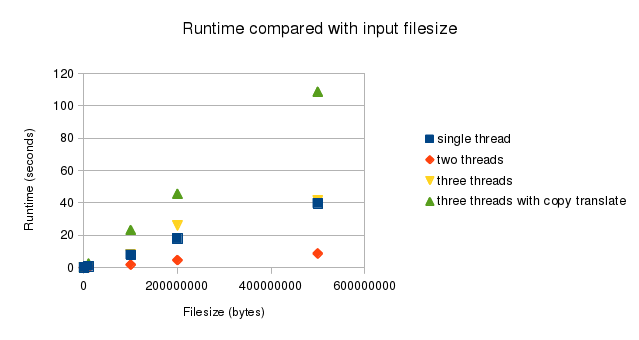
\includegraphics[width=1.2\textwidth]{graph.png}}
  \caption{Runtime Results}
\end{figure}

The results clearly show that care needs to be taken when breaking processes up into threads.
By using too many threads, it is possible to reduce the performance over a simple program with no threads.
The slowest performing program has to wait for both the input and the output thread to have free space in the buffers before it begins the translation process.
The fastest program will inflate data into a buffer in one thread and then translate and deflate data in the other thread.
This experiment did not make use of tools, such as Valgrind, to try measure which parts of the program were running the slowest.
Future work should characterise which parts of the program run the slowest and attempt to optimise those sections, possibly by exploiting parallelism.

\section{Conclusion}
Splitting programs into multiple threads can be an effective way of improving the program's performance.
The threads need to be carefully designed as it is possible to decrease the program performance by using poorly planned threads.

\newpage

\section{Appendix A - Program Code}
\subsection{One Thread}
\begin{minted}{c}
/*
 * This program will translate existing written works into a language
 * understandable by future generations. Input and output data are
 * compressed using gzip.
 *
 * Dan Collins 2014
 * COMP301 - 14B
 * 1183446
 */

#include <stdlib.h>
#include <stdio.h>
#include <zlib.h>

/* Maximum number of bytes to read from file */
#define BUF_SIZE 2048

/* Print program usage instructions */
void usage(char *name) {
  printf("Translator Usage\n");
  printf("%s input.gz output.gz\n", name);
}

/* Translate len characters in buf
 * a,A -> 4
 * e,E -> 3
 * i,I -> 1
 * o,O -> 0
 * s,S -> 5
 */
/* O(n) */
void translate(char *buf, int len) {
  int i;

  /* In place translation */
  for (i = 0; i < len; i++) {
    if (buf[i] == 'a' || buf[i] == 'A')
      buf[i] = '4';

    if (buf[i] == 'e' || buf[i] == 'E')
      buf[i] = '3';

    if (buf[i] == 'i' || buf[i] == 'I')
      buf[i] = '1';

    if (buf[i] == 'o' || buf[i] == 'O')
      buf[i] = '0';

    if (buf[i] == 's' || buf[i] == 'S')
      buf[i] = '5';
  }
}

int main(int argc, char **argv) {
  gzFile input, output;
  int len;
  char in_buf[BUF_SIZE];

  /* Test input arguments */
  if (argc != 3) {
    fprintf(stderr, "Invalid input arguments\n");
    usage(argv[0]);
    return -1;
  }

  /* Open input file */
  input = gzopen(argv[1], "rb");
  if (input == NULL) {
    fprintf(stderr, "Unable to open %s.\n", argv[1]);
    return -1;
  }

  /* Open output file */
  output = gzopen(argv[2], "wb");
  if (output == NULL) {
    fprintf(stderr, "Unable to open %s.\n", argv[2]);
    return -1;
  }

  /* Read all the bytes from the input file in chunks */
  while ((len = gzread(input, in_buf, BUF_SIZE)) > 0) {
    /* Translate the chunk */
    translate(in_buf, len);
    /* Write the translated data to the compressed output file */
    gzwrite(output, in_buf, len);
  }

  /* Close the files */
  gzclose(input);
  gzclose(output);

  return 0;
}
\end{minted}

\subsection{Two Threads}
\begin{minted}{c}
/*
 * This program will translate existing written works into a language
 * understandable by future generations. Input and output data are
 * compressed using gzip. The program itself makes use of threading
 * to leverage multiple CPUs commonly available.
 *
 * Dan Collins 2014
 * COMP301 - 14B
 * 1183446
 */

#include <stdlib.h>
#include <stdio.h>
#include <string.h>
#include <zlib.h>
#include <pthread.h>

/* Maximum number of bytes to read from file */
#define BUF_SIZE 2048

/* Threads will r/w from opposite buffers */
char in_buf_a[BUF_SIZE], in_buf_b[BUF_SIZE];
int in_len_a, in_len_b;
pthread_mutex_t in_mutex_a, in_mutex_b;

/* This will be set when the input file is EOF */
int eof;

/* Print program usage instructions */
void usage(char *name) {
  printf("Translator Usage\n");
  printf("%s input.gz output.gz\n", name);
}

/* Translate len characters in buf
 * a,A -> 4
 * e,E -> 3
 * i,I -> 1
 * o,O -> 0
 * s,S -> 5
 */
/* O(n) */
void translate(char *buf, int len) {
  int i;

  /* In place translation */
  for (i = 0; i < len; i++) {
    if (buf[i] == 'a' || buf[i] == 'A')
      buf[i] = '4';

    if (buf[i] == 'e' || buf[i] == 'E')
      buf[i] = '3';

    if (buf[i] == 'i' || buf[i] == 'I')
      buf[i] = '1';

    if (buf[i] == 'o' || buf[i] == 'O')
      buf[i] = '0';

    if (buf[i] == 's' || buf[i] == 'S')
      buf[i] = '5';
  }
}

void *translate_thread(void *args) {
  gzFile output = (gzFile)args;

  /* While the input thread is running, and there is data in the
   * buffers to translate... */
  while ((eof == 0) || (in_len_a > 0) || (in_len_b > 0)) {
    /* Wait until there is data in this buffer */
    if (in_len_a > 0) {
      pthread_mutex_lock(&in_mutex_a);

      /* We have the mutex, so translate the buffer safely */
      translate(in_buf_a, in_len_a);

      /* Write the translated data to the compressed output file */
      gzwrite(output, in_buf_a, in_len_a);

      /* This will tell the input thread this buffer is now empty */
      in_len_a = 0;
      pthread_mutex_unlock(&in_mutex_a);
    }
    
    /* Wait for the buffer to have data */
    if (in_len_b > 0) {
      pthread_mutex_lock(&in_mutex_b);

      /* Translate safely, as we have the mutex */
      translate(in_buf_b, in_len_b);

      /* Write the translated data to the compressed output file */
      gzwrite(output, in_buf_b, in_len_b);

      /* This will tell the input thread this buffer is now empty */
      in_len_b = 0;
      pthread_mutex_unlock(&in_mutex_b);
    }
  }

  /* No more data to translate, so we're done */
  pthread_exit(NULL);
}

int main(int argc, char **argv) {
  gzFile input, output;
  pthread_t trans, write;
  pthread_attr_t attr;
  int ret, len;
  char *ibuf; /* Will point to an input buffer */

  /* Test input arguments */
  if (argc != 3) {
    fprintf(stderr, "Invalid input arguments\n");
    usage(argv[0]);
    return -1;
  }

  /* Reset buffers */
  in_len_a = 0; in_len_b = 0;

  /* Clear EOF flag */
  eof = 0;

  /* Open input file */
  input = gzopen(argv[1], "rb");
  if (input == NULL) {
    fprintf(stderr, "Unable to open %s.\n", argv[1]);
    return -1;
  }

  /* Open output file */
  output = gzopen(argv[2], "wb");
  if (output == NULL) {
    fprintf(stderr, "Unable to open %s.\n", argv[2]);
    return -1;
  }

  /* Create the mutexes */
  pthread_mutex_init(&in_mutex_a, NULL);
  pthread_mutex_init(&in_mutex_b, NULL);

  /* Configure attributes for the threads */
  pthread_attr_init(&attr);
  pthread_attr_setstacksize(&attr, 2 * 1000 * 1000); /* 2MB */
  pthread_attr_setdetachstate(&attr, PTHREAD_CREATE_JOINABLE);

  /* Create and start the translation and output thread */
  ret = pthread_create(&trans, NULL, translate_thread, NULL);
  if (ret != 0) {
    fprintf(stderr, "Failed to create translate thread: %d\n", ret);
    return -1;
  }

  /* Read data in chunks to alternating input buffers.
   * The data will get used by the translate thread */
  while (!gzeof(input)) {
    pthread_mutex_lock(&in_mutex_a);
    if (in_len_a == 0) {
      len = gzread(input, in_buf_a, BUF_SIZE);
      in_len_a = len;
    }
    pthread_mutex_unlock(&in_mutex_a);
    
    pthread_mutex_lock(&in_mutex_b);
    if (in_len_b == 0) {
      len = gzread(input, in_buf_b, BUF_SIZE);
      in_len_b = len;
    }
    pthread_mutex_unlock(&in_mutex_b);
  }

  /* Notify other threads that EOF has occured */
  eof = 1;

  /* Block until all threads are done */
  pthread_join(trans, NULL);

  /* Clear the mutexes */
  pthread_mutex_destroy(&in_mutex_a);
  pthread_mutex_destroy(&in_mutex_b);

  /* Clear the attribute memory */
  pthread_attr_destroy(&attr);

  /* Close the files */
  gzclose(input);
  gzclose(output);

  return 0;
}
\end{minted}

\subsection{Three Threads}
\begin{minted}{c}
/*
 * This program will translate existing written works into a language
 * understandable by future generations. Input and output data are
 * compressed using gzip. The program itself makes use of threading
 * to leverage multiple CPUs commonly available.
 *
 * Dan Collins 2014
 * COMP301 - 14B
 * 1183446
 */

#include <stdlib.h>
#include <stdio.h>
#include <string.h>
#include <zlib.h>
#include <pthread.h>

/* Maximum number of bytes to read from file */
#define BUF_SIZE 2048

/* Threads will r/w from opposite buffers */
char in_buf_a[BUF_SIZE], in_buf_b[BUF_SIZE];
int in_len_a, in_len_b;
pthread_mutex_t in_mutex_a, in_mutex_b;

char out_buf_a[BUF_SIZE], out_buf_b[BUF_SIZE];
int out_len_a, out_len_b;
pthread_mutex_t out_mutex_a, out_mutex_b;

/* This will be set when the input file is EOF */
int eof;
/* This will be set when the translation is done */
int trans_done;

/* Print program usage instructions */
void usage(char *name) {
  printf("Translator Usage\n");
  printf("%s input.gz output.gz\n", name);
}

/* Translate len characters in buf
 * a,A -> 4
 * e,E -> 3
 * i,I -> 1
 * o,O -> 0
 * s,S -> 5
 */
/* O(n) */
void translate(char *buf, int len) {
  int i;

  /* In place translation */
  for (i = 0; i < len; i++) {
    if (buf[i] == 'a' || buf[i] == 'A')
      buf[i] = '4';

    if (buf[i] == 'e' || buf[i] == 'E')
      buf[i] = '3';

    if (buf[i] == 'i' || buf[i] == 'I')
      buf[i] = '1';

    if (buf[i] == 'o' || buf[i] == 'O')
      buf[i] = '0';

    if (buf[i] == 's' || buf[i] == 'S')
      buf[i] = '5';
  }
}

void *translate_thread(void *args) {
  /* While the input thread is running, and there is data in the
   * buffers to translate... */
  while ((eof == 0) || (in_len_a > 0) || (in_len_b > 0)) {
    /* Wait until there is data in this buffer */
    if (in_len_a > 0) {
      pthread_mutex_lock(&in_mutex_a);

      /* Translate the data in-place */
      translate(in_buf_a, in_len_a);

      /* We also need to copy into the output buffer, which needs to
       * be available and empty */
      while (out_len_a > 0)
	;
      pthread_mutex_lock(&out_mutex_a);
      memcpy(out_buf_a, in_buf_a, in_len_a);
      out_len_a = in_len_a;
      pthread_mutex_unlock(&out_mutex_a);

      /* This will tell the input thread this buffer is now empty */
      in_len_a = 0;
      pthread_mutex_unlock(&in_mutex_a);
    }
    
    /* Wait for the buffer to have data */
    if (in_len_b > 0) {
      pthread_mutex_lock(&in_mutex_b);

      /* Translate the data in-place */
      translate(in_buf_a, in_len_a);

      /* Wait until there is room for the output data */
      while (out_len_b > 0)
	;
      pthread_mutex_lock(&out_mutex_b);
      /* Copy the translated data */
      memcpy(out_buf_b, in_buf_b, in_len_b);
      out_len_b = in_len_b;
      pthread_mutex_unlock(&out_mutex_b);

      /* This will tell the input thread this buffer is now empty */
      in_len_b = 0;
      pthread_mutex_unlock(&in_mutex_b);
    }
  }

  /* No more data to translate, so we're done */
  trans_done = 1;
  pthread_exit(NULL);
}

void *write_thread(void *args) {
  gzFile output = (gzFile)args;

  /* While the translate thread is still running, and there is data
   * to output... */
  while ((trans_done == 0) || (out_len_a > 0) || (out_len_b > 0)) {
    if (out_len_a > 0) {
      pthread_mutex_lock(&out_mutex_a);

      /* Write the translated data to the compressed output file */
      gzwrite(output, out_buf_a, out_len_a);

      /* Tell the translate thread we're done with the data */
      out_len_a = 0;
      pthread_mutex_unlock(&out_mutex_a);
    }

    if (out_len_b > 0) {
      pthread_mutex_lock(&out_mutex_b);

      /* Write the translated data to the compressed output file */
      gzwrite(output, out_buf_b, out_len_b);

      /* Tell the translate thread we're done with the data */
      out_len_b = 0;
      pthread_mutex_unlock(&out_mutex_b);
    }
  }

  pthread_exit(NULL);
}

int main(int argc, char **argv) {
  gzFile input, output;
  pthread_t trans, write;
  pthread_attr_t attr;
  int ret, len;
  char *ibuf; /* Will point to an input buffer */

  /* Test input arguments */
  if (argc != 3) {
    fprintf(stderr, "Invalid input arguments\n");
    usage(argv[0]);
    return -1;
  }

  /* Reset buffers */
  in_len_a = 0; in_len_b = 0;
  out_len_a = 0; out_len_b = 0;

  /* Clear EOF flag */
  eof = 0;
  /* Clear translate flag */
  trans_done = 0;

  /* Open input file */
  input = gzopen(argv[1], "rb");
  if (input == NULL) {
    fprintf(stderr, "Unable to open %s.\n", argv[1]);
    return -1;
  }

  /* Open output file */
  output = gzopen(argv[2], "wb");
  if (output == NULL) {
    fprintf(stderr, "Unable to open %s.\n", argv[2]);
    return -1;
  }

  /* Create the mutexes */
  pthread_mutex_init(&in_mutex_a, NULL);
  pthread_mutex_init(&in_mutex_b, NULL);
  pthread_mutex_init(&out_mutex_a, NULL);
  pthread_mutex_init(&out_mutex_b, NULL);

  /* Configure attributes for the threads */
  pthread_attr_init(&attr);
  pthread_attr_setstacksize(&attr, 2 * 1000 * 1000); /* 2MB */
  pthread_attr_setdetachstate(&attr, PTHREAD_CREATE_JOINABLE);

  /* Create and start the translation and output threads */
  ret = pthread_create(&trans, NULL, translate_thread, NULL);
  if (ret != 0) {
    fprintf(stderr, "Failed to create translate thread: %d\n", ret);
    return -1;
  }

  ret = pthread_create(&write, NULL, write_thread, (void *)output);
  if (ret != 0) {
    fprintf(stderr, "Failed to create output thread: %d\n", ret);
    return -1;
  }

  /* Read data in chunks to alternating input buffers.
   * The data will get used by the translate thread */
  while (!gzeof(input)) {
    pthread_mutex_lock(&in_mutex_a);
    if (in_len_a == 0) {
      len = gzread(input, in_buf_a, BUF_SIZE);
      in_len_a = len;
    }
    pthread_mutex_unlock(&in_mutex_a);
    
    pthread_mutex_lock(&in_mutex_b);
    if (in_len_b == 0) {
      len = gzread(input, in_buf_b, BUF_SIZE);
      in_len_b = len;
    }
    pthread_mutex_unlock(&in_mutex_b);
  }

  /* Notify other threads that EOF has occured */
  eof = 1;

  /* Block until all threads are done */
  pthread_join(trans, NULL);
  pthread_join(write, NULL);

  /* Clear the mutexes */
  pthread_mutex_destroy(&in_mutex_a);
  pthread_mutex_destroy(&in_mutex_b);
  pthread_mutex_destroy(&out_mutex_a);
  pthread_mutex_destroy(&out_mutex_b);

  /* Clear the attribute memory */
  pthread_attr_destroy(&attr);

  /* Close the files */
  gzclose(input);
  gzclose(output);

  return 0;
}
\end{minted}

\subsection{Three Threads - Copying Translate}
\begin{minted}{c}
/*
 * This program will translate existing written works into a language
 * understandable by future generations. Input and output data are
 * compressed using gzip. The program itself makes use of threading
 * to leverage multiple CPUs commonly available.
 *
 * Dan Collins 2014
 * COMP301 - 14B
 * 1183446
 */

#include <stdlib.h>
#include <stdio.h>
#include <string.h>
#include <zlib.h>
#include <pthread.h>

/* Maximum number of bytes to read from file */
#define BUF_SIZE 2048

/* Threads will r/w from opposite buffers */
char in_buf_a[BUF_SIZE], in_buf_b[BUF_SIZE];
int in_len_a, in_len_b;
pthread_mutex_t in_mutex_a, in_mutex_b;

char out_buf_a[BUF_SIZE], out_buf_b[BUF_SIZE];
int out_len_a, out_len_b;
pthread_mutex_t out_mutex_a, out_mutex_b;

/* This will be set when the input file is EOF */
int eof;
/* This will be set when the translation is done */
int trans_done;

/* Print program usage instructions */
void usage(char *name) {
  printf("Translator Usage\n");
  printf("%s input.gz output.gz\n", name);
}

/* Translate len characters in buf
 * a,A -> 4
 * e,E -> 3
 * i,I -> 1
 * o,O -> 0
 * s,S -> 5
 */
/* O(n) */
void translate(char *buf, int len) {
  int i;

  /* In place translation */
  for (i = 0; i < len; i++) {
    if (buf[i] == 'a' || buf[i] == 'A')
      buf[i] = '4';

    if (buf[i] == 'e' || buf[i] == 'E')
      buf[i] = '3';

    if (buf[i] == 'i' || buf[i] == 'I')
      buf[i] = '1';

    if (buf[i] == 'o' || buf[i] == 'O')
      buf[i] = '0';

    if (buf[i] == 's' || buf[i] == 'S')
      buf[i] = '5';
  }
}

/* Same translation as above, but will copy at the same time */
void translate_copy(char *dest, char *src, int len) {
  int i;

  for (i = 0; i < len; i++) {
    if (src[i] == 'a' || src[i] == 'A')
      dest[i] = '4';

    if (src[i] == 'e' || src[i] == 'E')
      dest[i] = '3';

    if (src[i] == 'i' || src[i] == 'I')
      dest[i] = '1';

    if (src[i] == 'o' || src[i] == 'O')
      dest[i] = '0';

    if (src[i] == 's' || src[i] == 'S')
      dest[i] = '5';
  }
}

void *translate_thread(void *args) {
  /* While the input thread is running, and there is data in the
   * buffers to translate... */
  while ((eof == 0) || (in_len_a > 0) || (in_len_b > 0)) {
    /* Wait until there is data in this buffer */
    if (in_len_a > 0) {
      pthread_mutex_lock(&in_mutex_a);

      /* We also need to copy into the output buffer, which needs to
       * be available and empty */
      while (out_len_a > 0)
	;
      pthread_mutex_lock(&out_mutex_a);
      /* Translate away */
      translate_copy(out_buf_a, in_buf_a, in_len_a);
      out_len_a = in_len_a;
      pthread_mutex_unlock(&out_mutex_a);

      /* This will tell the input thread this buffer is now empty */
      in_len_a = 0;
      pthread_mutex_unlock(&in_mutex_a);
    }
    
    /* Wait for the buffer to have data */
    if (in_len_b > 0) {
      pthread_mutex_lock(&in_mutex_b);

      /* Wait until there is room for the output data */
      while (out_len_b > 0)
	;
      pthread_mutex_lock(&out_mutex_b);
      /* Copy the translated data */
      translate_copy(out_buf_b, in_buf_b, in_len_b);
      out_len_b = in_len_b;
      pthread_mutex_unlock(&out_mutex_b);

      /* This will tell the input thread this buffer is now empty */
      in_len_b = 0;
      pthread_mutex_unlock(&in_mutex_b);
    }
  }

  /* No more data to translate, so we're done */
  trans_done = 1;
  pthread_exit(NULL);
}

void *write_thread(void *args) {
  gzFile output = (gzFile)args;

  /* While the translate thread is still running, and there is data
   * to output... */
  while ((trans_done == 0) || (out_len_a > 0) || (out_len_b > 0)) {
    if (out_len_a > 0) {
      pthread_mutex_lock(&out_mutex_a);

      /* Write the translated data to the compressed output file */
      gzwrite(output, out_buf_a, out_len_a);

      /* Tell the translate thread we're done with the data */
      out_len_a = 0;
      pthread_mutex_unlock(&out_mutex_a);
    }

    if (out_len_b > 0) {
      pthread_mutex_lock(&out_mutex_b);

      /* Write the translated data to the compressed output file */
      gzwrite(output, out_buf_b, out_len_b);

      /* Tell the translate thread we're done with the data */
      out_len_b = 0;
      pthread_mutex_unlock(&out_mutex_b);
    }
  }

  pthread_exit(NULL);
}

int main(int argc, char **argv) {
  gzFile input, output;
  pthread_t trans, write;
  pthread_attr_t attr;
  int ret, len;
  char *ibuf; /* Will point to an input buffer */

  /* Test input arguments */
  if (argc != 3) {
    fprintf(stderr, "Invalid input arguments\n");
    usage(argv[0]);
    return -1;
  }

  /* Reset buffers */
  in_len_a = 0; in_len_b = 0;
  out_len_a = 0; out_len_b = 0;

  /* Clear EOF flag */
  eof = 0;
  /* Clear translate flag */
  trans_done = 0;

  /* Open input file */
  input = gzopen(argv[1], "rb");
  if (input == NULL) {
    fprintf(stderr, "Unable to open %s.\n", argv[1]);
    return -1;
  }

  /* Open output file */
  output = gzopen(argv[2], "wb");
  if (output == NULL) {
    fprintf(stderr, "Unable to open %s.\n", argv[2]);
    return -1;
  }

  /* Create the mutexes */
  pthread_mutex_init(&in_mutex_a, NULL);
  pthread_mutex_init(&in_mutex_b, NULL);
  pthread_mutex_init(&out_mutex_a, NULL);
  pthread_mutex_init(&out_mutex_b, NULL);

  /* Configure attributes for the threads */
  pthread_attr_init(&attr);
  pthread_attr_setstacksize(&attr, 2 * 1000 * 1000); /* 2MB */
  pthread_attr_setdetachstate(&attr, PTHREAD_CREATE_JOINABLE);

  /* Create and start the translation and output threads */
  ret = pthread_create(&trans, NULL, translate_thread, NULL);
  if (ret != 0) {
    fprintf(stderr, "Failed to create translate thread: %d\n", ret);
    return -1;
  }

  ret = pthread_create(&write, NULL, write_thread, (void *)output);
  if (ret != 0) {
    fprintf(stderr, "Failed to create output thread: %d\n", ret);
    return -1;
  }

  /* Read data in chunks to alternating input buffers.
   * The data will get used by the translate thread */
  while (!gzeof(input)) {
    pthread_mutex_lock(&in_mutex_a);
    if (in_len_a == 0) {
      len = gzread(input, in_buf_a, BUF_SIZE);
      in_len_a = len;
    }
    pthread_mutex_unlock(&in_mutex_a);
    
    pthread_mutex_lock(&in_mutex_b);
    if (in_len_b == 0) {
      len = gzread(input, in_buf_b, BUF_SIZE);
      in_len_b = len;
    }
    pthread_mutex_unlock(&in_mutex_b);
  }

  /* Notify other threads that EOF has occured */
  eof = 1;

  /* Block until all threads are done */
  pthread_join(trans, NULL);
  pthread_join(write, NULL);

  /* Clear the mutexes */
  pthread_mutex_destroy(&in_mutex_a);
  pthread_mutex_destroy(&in_mutex_b);
  pthread_mutex_destroy(&out_mutex_a);
  pthread_mutex_destroy(&out_mutex_b);

  /* Clear the attribute memory */
  pthread_attr_destroy(&attr);

  /* Close the files */
  gzclose(input);
  gzclose(output);

  return 0;
}
\end{minted}

\end{document}
